\documentclass{article}
\usepackage{graphicx} % Required for inserting images
\usepackage{tikz}
\usetikzlibrary{positioning, arrows.meta, fit, backgrounds}

\title{Computer Architecture - Final Report}
\author{s255299, s255, s255}
\date{November 2026}

\begin{document}

\maketitle

\section{Introduction}
\section{design}
\subsection{Program Structure}
The simulator is split into three main structs: a \verb|FileHandler|,
a \verb|ProgramCounter| and an \verb|InstructionHandler|. The program does
not follow a specific software architecture, but is mostly built in an
object-oriented style: each component is a simple C struct whose functions are
stored as function pointers, so they behave like methods on an object.
The \verb|main| function is the entrypoint of the program. It reads the binary program
into memory, then repeatedly fetches the instruction at the current program
counter, decodes and executes it, and advances the counter.

\begin{itemize}
    \item \textbf{FileHandler} - reads the input binary file and returns
          the program as an array of 32-bit instructions.
    \item \textbf{ProgramCounter} - keeps track of the address of the
          current instruction and increments it by 4 after each step.
    \item \textbf{InstructionHandler} - holds the 32 registers, decodes each
          instruction into its corresponding field (\verb|rd, rs1, rs2, funct3, funct7|) and executes it.
\end{itemize}
\begin{figure}[htbp]
\centering
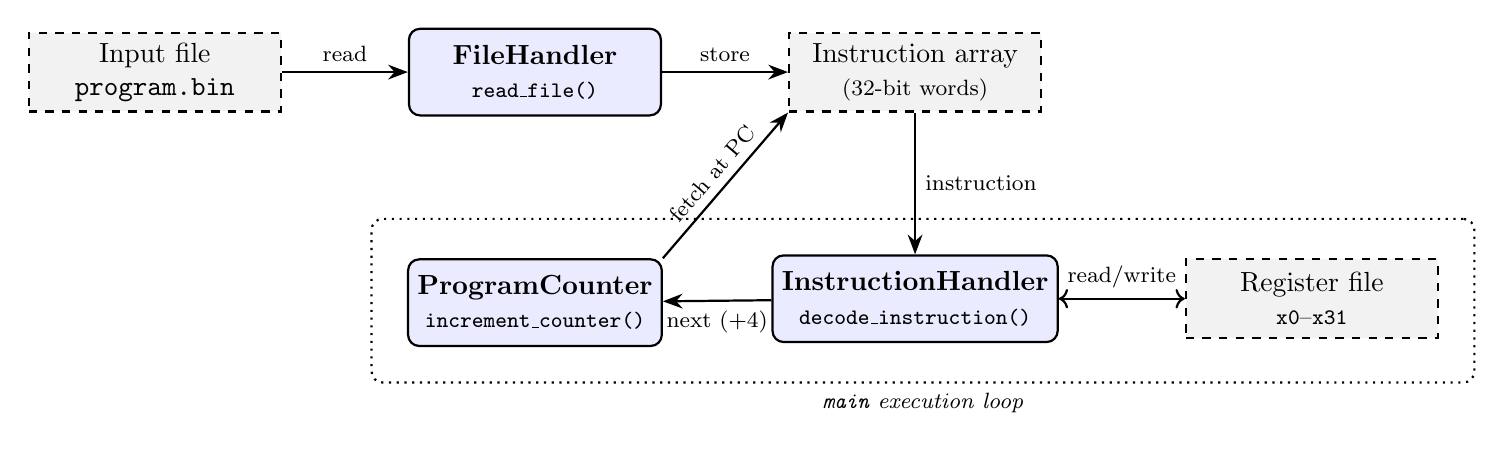
\begin{tikzpicture}[
    node distance = 1.2cm and 1.6cm,
    block/.style  = {rectangle, draw, thick, rounded corners,
                     minimum width=3.2cm, minimum height=1.1cm,
                     align=center, fill=blue!8},
    data/.style   = {rectangle, draw, dashed, thick,
                     minimum width=3.2cm, minimum height=1.0cm,
                     align=center, fill=gray!10},
    arrow/.style  = {-{Stealth[length=2.5mm]}, thick},
    lbl/.style    = {font=\footnotesize, midway}
]

% Nodes
\node[data]  (bin)  {Input file\\\texttt{program.bin}};
\node[block, right=of bin] (fh) {\textbf{FileHandler}\\\footnotesize\texttt{read\_file()}};
\node[data,  right=of fh]  (mem) {Instruction array\\\footnotesize(32-bit words)};

\node[block, below=1.8cm of mem] (ih)
     {\textbf{InstructionHandler}\\\footnotesize\texttt{decode\_instruction()}};
\node[data,  right=of ih] (reg) {Register file\\\footnotesize\texttt{x0}--\texttt{x31}};
\node[block, below=1.8cm of fh] (pc)
     {\textbf{ProgramCounter}\\\footnotesize\texttt{increment\_counter()}};

% Load phase
\draw[arrow] (bin) -- node[lbl, above] {read} (fh);
\draw[arrow] (fh)  -- node[lbl, above] {store} (mem);

% Execution loop
\draw[arrow] (pc.north east) -- node[lbl, sloped, above] {fetch at PC} (mem.south west);
\draw[arrow] (mem) -- node[lbl, right] {instruction} (ih);
\draw[arrow, <->] (ih) -- node[lbl, above] {read/write} (reg);
\draw[arrow] (ih) -- node[lbl, below] {next ($+4$)} (pc);

% Main loop frame
\begin{scope}[on background layer]
  \node[draw, thick, dotted, rounded corners, inner sep=0.45cm,
        fit=(pc) (ih) (reg),
        label={[font=\footnotesize\itshape]below:\texttt{main} execution loop}] {};
\end{scope}

\end{tikzpicture}
\caption{Program structure of the simulator. The \texttt{FileHandler} loads
the binary into memory once. The \texttt{ProgramCounter} and
\texttt{InstructionHandler} then run the fetch--decode--execute loop.}
\label{fig:program-structure}
\end{figure}

\section{implementation}
\section{discussion}

\end{document}
